\documentclass{beamer}
%% apparently this magic helps avoid the dreaded
%% ``Too many math alphabets used in version normal''
%% error. Yuk.
\newcommand\hmmax{0}
\newcommand\bmmax{0}
%% end magic

\usepackage{amssymb,amsmath,amsthm}
\usepackage{latexsym}

\usepackage{array}

\usepackage{url}
\usepackage{hyperref}

%% uses the AMS Euler math font.
\usepackage{euler}

%% for coloneqq
%% \usepackage{mathtools}

%% for \underaccent
\usepackage{accents}

% for semantic brackets
%% \usepackage{stmaryrd}

% for inference rules
\usepackage{proof}

%% for mathpar environment
\usepackage{mathpartir}

% for \scalebox, \rotatebox
%% \usepackage{graphicx}

%% for colors
\usepackage{color}

%% for drawing Hasse diagram
\usepackage{tikz}

%% for censoring things
\usepackage{censor}


%% Commands
\newcommand{\mto}{\overset{+\:}{\to}}
\newcommand{\eq}[1]{\underaccent{\mathit{eq}}{#1}}
\newcommand{\fin}[1]{\underaccent{\mathit{fin}}{#1}}
\newcommand{\m}[1]{\ensuremath{\mathbf{#1}}}
\newcommand{\ms}{\mathsf}


%% Metadata
\title{Datafun}
\author{Michael Arntzenius\inst{1} \and Neel Krishnaswami\inst{2}}
\institute{\inst{1}University of Birmingham \and \inst{2}University of Cambridge}
\date{ICFP 2016}


\begin{document}

\maketitle

\begin{frame}
  \frametitle{What is Datafun?}

  Datafun is a \emph{pure}, \emph{total} functional language for expressing
  \textbf{fixed points} of \textbf{monotone maps} on \textbf{semilattices}
  satisfying an \textbf{ascending chain condition}.

  \vspace{1.5em}

  Example: \textbf{Static analysis!}
\end{frame}

\begin{frame}
  \frametitle{Static analysis}

  \begin{tabular}{rl}
    1 & \texttt{\censor{x := 0}}\\
    2 & \texttt{\censor{t := 3}}\\
    3 & \texttt{\censor{while true do}}\\
    4 & \texttt{\quad \censor{s := if x = 0 then 7 else 4 + t}}\\
    5 & \texttt{\quad \censor{x $\leftarrow$ x + 1}}\\
    6 & \texttt{\quad print s} \qquad {\small \texttt{\#} can be replaced by \texttt{print 7}}
  \end{tabular}
\end{frame}


\begin{frame}
  \frametitle{Static analysis}

  \begin{tabular}{rll}
    1 & \texttt{x := 0} & x = 0\\
    2 & \texttt{\alt<2->{t := 3}{\censor{t := 3}}}
      & \uncover<2->{x = 0, t = 3}\\
    3 & \texttt{\alt<3->{while true do}{\censor{while true do}}}
      & \uncover<3->{x = 0, t = 3}\\
    4 & \texttt{\quad \alt<4->{s := if x = 0 then 7 else 4 + t}
                              {\censor{s := if x = 0 then 7 else 4 + t}}}
      & \uncover<4->{x = 0, t = 3, s = \alt<5->{7}{\color{red}{?}}}\\
    5 & \texttt{\quad \alt<6->{x $\leftarrow$ x + 1}
                              {\censor{x $\leftarrow$ x + 1}}}
      & \uncover<6->{x = \alt<7->{1}{{\color{red}?}}, t = 3, s = 7}\\
    6 & \texttt{\quad print s}
      & \uncover<8->{x = 1, t = 3, s = 7}
  \end{tabular}
\end{frame}

\begin{frame}
  \frametitle{Static analysis}

  \begin{tabular}{rll}
    1 & \texttt{x := 0} & x = 0\\
    2 & \texttt{t := 3} & x = 0, t = 3\\
    \color<1,7>{red}
    3 & \texttt{\color<1,7>{red} while true do}
      & {\color<1,7>{red} x = $\top$, t = 3}\\
    \color<1>{gray}\color<2-4>{red}
    4 & \color<1>{gray}\color<2-4>{red}
        \texttt{\quad s := if x = 0 then 7 else 4 + t}
      & \color<1>{gray}\color<2-4>{red}
        x = \alt<3->{$\top$}{{\color<2>{gray}0}}, t = 3, s = {\color<2-3>{gray}7}\\
    \color<1-4>{gray}\color<5>{red}
    5 & \color<1-4>{gray}\color<5>{red}
        \texttt{\quad x $\leftarrow$ x + 1}
      & \color<1-4>{gray}\color<5>{red}
        x = \alt<5->{$\top$}{1}, t = 3, s = 7\\
    \color<1-5>{gray}\color<6>{red}\color<8>{blue}
    6 & \color<1-5>{gray}\color<6>{red}\color<8>{blue} \texttt{\quad print s}
      & \color<1-5>{gray}\color<6>{red}\color<8>{blue}
        x = \alt<6->{$\top$}{1}, t = 3, s = 7
  \end{tabular}
\end{frame}


\begin{frame}
  \frametitle{What about our definition?}

  {\footnotesize\color{gray} Datafun is a \emph{pure}, \emph{total} functional
    language for expressing \textbf{\color{black} fixed points} of
    \textbf{\color{black} monotone maps} on \textbf{\color{black} semilattices}
    satisfying an \textbf{\color{black} ascending chain condition}.}

  \vspace{0.5em}

  \begin{itemize}
  \item \textbf{Semilattice}:\\

    \begin{center}
      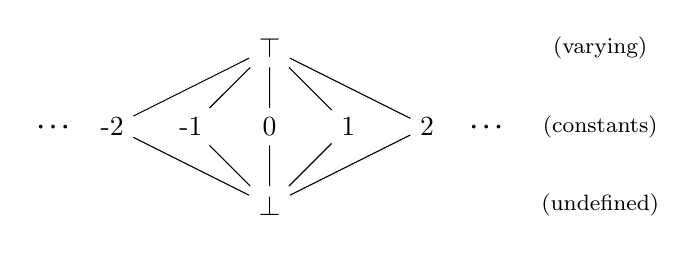
\begin{tikzpicture}[scale=1]
        \node (top)  at ( 0, 1) {$\top$};
        \node (bot)  at ( 0,-1) {$\bot$};
        \node (-3)   at (-2.75, 0) {$\hdots$};
        \node (-2)   at (-2, 0) {-2};
        \node (-1)   at (-1, 0) {-1};
        \node (0)    at ( 0, 0) {0};
        \node (1)    at ( 1, 0) {1};
        \node (2)    at ( 2, 0) {2};
        \node (3)    at ( 2.75, 0) {$\hdots$};
        %% TODO: left-align these
        \node (varying)   at (4.2, 1) {\footnotesize (varying)};
        \node (constant)  at (4.2, 0) {\footnotesize (constants)};
        \node (undefined) at (4.2,-1) {\footnotesize (undefined)};
        \draw (bot) -- (-2) -- (top) -- (-1) -- (bot) -- (0) -- (top)
        -- (1) -- (bot) -- (2) -- (top);
      \end{tikzpicture}
    \end{center}

  \item \textbf{Monotone}: Only go \emph{up}: $\bot \Rightarrow \text{constant} \Rightarrow \top$
  \item \textbf{Ascending chain condition}: Can't go up forever.
  \item \textbf{Fixed point}: Keep going until nothing changes.
  \end{itemize}

\end{frame}


\begin{frame}
  \frametitle{What else fits this mold?}

  \begin{itemize}
  \item Static analyses
  \item Graph reachability, connectedness, shortest path, \&c
  \item CYK algorithm for CFG parsing
  \item \textbf{Every Datalog program}
  \end{itemize}
\end{frame}


\begin{frame}
  \frametitle{How do we express semilattice fixed points?}

  To the simply-typed lambda calculus, add...\pause

  {\huge\[ \alt<3->{\ms{fix}\;\m{x}\;\ms{is}\;[...]}
                   {\ms{fix}\;(\lambda \m{x}.\; [...])} \]}\pause\pause

  Need to check:
  \begin{enumerate}
  \item That $(\lambda \m{x}.\; [...])$ is a \textbf{monotone} function
  \item \color{gray} on a \textbf{semilattice} satisfying \textbf{ACC}.
  \end{enumerate}

\end{frame}

\begin{frame}
  \begin{center}
    \huge\bf Track monotonicity with types!
  \end{center}
\end{frame}

\begin{frame}
  \frametitle{Types as posets}
  \begin{center}
    \begin{tabular}{cll}
      \textbf{Type} & \textbf{Meaning} & \textbf{Ordering}
      \\\hline
      $2$ & booleans & $\ms{false} < \ms{true}$\\
      $A \times B$ & pairs & pointwise\\
      $\{A\}$      & finite sets & by inclusion: $x \le y \iff x \subseteq y$\\
      %% $\ms{Flat}\;A$ &
      %% %% an $A$ or $\bot$ or $\top$ &
      %% \multicolumn{2}{m{4cm}}{\scriptsize
      %%   \begin{tikzpicture}[scale=0.5]
      %%   \node (top)  at ( 0, 1) {$\top$};
      %%   \node (bot)  at ( 0,-1) {$\bot$};
      %%   \node (-2)   at (-1.49, 0) {$\hdots$};
      %%   \node (-1)   at (-0.75, 0) {$\hdots$};
      %%   \node (0)    at ( 0, 0) {$A$};
      %%   \node (1)    at (0.75, 0) {$\hdots$};
      %%   \node (2)    at (1.49, 0) {$\hdots$};
      %%   \draw (bot) -- (-2) -- (top) -- (-1) -- (bot) -- (0) --
      %%         (top) -- (1) -- (bot) -- (2) -- (top);
      %% \end{tikzpicture}}\\
      $A \to B$    & functions & pointwise\\
      $A \mto B$  & \textbf{monotone} functions & pointwise\\
    \end{tabular}
  \end{center}

  \vspace{0.75em}\pause

  \[\begin{array}{l}
    member ~:~ \mathbb{N} \to \{\mathbb{N}\} \mto 2\\
    member\; x\; \mathbf{s} = \exists(y \in \mathbf{s})\; x = y
  \end{array}\]

  \vspace{5em}

\end{frame}

%% monotone vs discrete
%% example: set membership
\begin{frame}
  \frametitle{Discrete vs monotone}

  %% Comment this list out and just speak it?
  \begin{itemize}
  \item Two types of \emph{function}: discrete or monotone
  \item Two kinds of \emph{variable}: discrete or monotone
  \item Two \emph{typing contexts}: $\Delta$ discrete, $\Gamma$ monotone
  \end{itemize}

  {\Large\[\Delta;\Gamma \vdash e : A\]}

  \begin{quote}
    \hspace{-1.1ex}``$e$ has type $A$ with free variables $\Delta,\Gamma$;\\
    moreover, $e$ is monotone in the variables in $\Gamma$.''
  \end{quote}
\end{frame}


\begin{frame}
  \frametitle{Typing rules: discrete vs monotone}

  {
  \begin{mathpar}
    \infer[\textsc{\footnotesize monotone app}]
          {\Delta;\Gamma \vdash f\, a : B}
          { \Delta;\Gamma \vdash f : A \mto B \hspace{1em}&
            {\color<2->{red}\Delta;\Gamma} \vdash a : A }
    \pause\vspace{1.25em}

    \infer[\textsc{\footnotesize discrete app}]
          {\Delta;\Gamma \vdash f\, a : B}
          { \Delta;\Gamma \vdash f : A \to B \hspace{1em}&
            {\color{red}\Delta;\cdot} \vdash a : A }
  \end{mathpar}
  }

  %% \color<2>{gray}\color<3>{black}
  Otherwise:
  \[\begin{array}{l}
  coerce ~:~ (\mathbb{N} \to \mathbb{N}) \to (\mathbb{N} \mto \mathbb{N})\\
  coerce\; f\; \mathbf{x} = f\; {\color{red}\mathbf{x}}
  \end{array}\]
  This shouldn't type-check!

%% Δ;Γ ⊢ e₁ : A →⁺ B    Δ;Γ ⊢ e₂ : A
%% ----------------------------------
%%       Δ;Γ ⊢ e₁ e₂ : B

\end{frame}


\begin{frame}
  \frametitle{Examples}

  \textbf{Relational composition:}\vspace{-0.8em}
  \[\begin{array}{l}
    (\bullet) : \{A \times \eq{B}\} \mto \{\eq{B} \times C\} \mto \{A \times C\}\\
    \m{s} \bullet \m{t} =
    \{(x,z) ~|~ (x,y) \in \m{s}, (!y,z) \in \m{t}\}
  \end{array}\]

  \vspace{0.2em}

  \textbf{Reachability:}\vspace{-0.8em}
  \[\begin{array}{l}
    path ~:~ \{\fin{A} \times \fin{A}\} \mto \{\fin{A} \times \fin{A}\}\\
    path\;\m{E} = \ms{fix}~\m{P}~\ms{is}~ \m{E} \cup (\m{P} \bullet \m{P})
  \end{array}\]
  \vspace{0.2em}

  In Datalog, for comparison:
  \begin{tabular}{l}
    \texttt{path(X,Y) :- edge(X,Y).}\\
    \texttt{path(X,Z) :- path(X,Y), path(Y,Z).}\\
  \end{tabular}

\end{frame}


\begin{frame}
  \frametitle{Summary}

  \begin{itemize}
  \item Many algorithms are concisely expressed as \textbf{fixed points} of
    \textbf{monotone maps} on \textbf{semilattices}
  \item We can represent semilattices as types
  \item We can track \textbf{monotonicity} with types, too!
  \end{itemize}

  \vspace{1em}
  \begin{center}
    {\Large \url{github.com/rntz/datafun}}
  \end{center}
\end{frame}

\end{document}
